\documentclass[12pt]{report}
\usepackage{graphicx}
\usepackage{hyperref}
\usepackage{setspace}
\usepackage{amsmath}
\usepackage{enumitem}
\usepackage{float}
\usepackage{subcaption}
\usepackage{multirow}
\usepackage{adjustbox}
\usepackage{textcomp}
\usepackage{lipsum}
\usepackage{color}
\usepackage{sectsty}
\usepackage[nottoc]{tocbibind}
\usepackage{grffile}
\usepackage{fancyhdr}
\usepackage{acro}
\usepackage[a4paper,includeheadfoot,margin=2.5cm]{geometry}
\pagestyle{fancy}
\usepackage{titlesec}
\usepackage{graphicx}
\usepackage{xcolor}
\usepackage{dirtree}
\usepackage{amssymb}
\usepackage{tikz}
\usepackage{pgfplots}
\graphicspath{{images/}}
\renewcommand{\headrulewidth}{0pt}
\usepackage{listings}
\usepackage{algorithm}
\usepackage[noend]{algpseudocode}
\usepackage{tabu}
\usepackage[scientific-notation=true]{siunitx}
\usepackage{hyperref}
\usepackage{microtype}
\usepackage{tikzsymbols}
\usepackage{makecell}
\usetikzlibrary{matrix,chains,positioning,decorations,arrows}
\emergencystretch=1em
\newcolumntype{M}[1]{>{\centering\arraybackslash}m{#1}}
\newlist{steps}{enumerate}{1}
\setlist[steps, 1]{label = Step \arabic*:}
\newcommand\myicon[1]{{\color{#1}\rule{2ex}{2ex}}}
\newcommand{\myfolder}[2]{\myicon{#1}\ {#2}}

%New colors defined below
\definecolor{codegreen}{rgb}{0,0.6,0}
\definecolor{codegray}{rgb}{0.5,0.5,0.5}
\definecolor{codeyellow}{rgb}{0.85, 0.65, 0.13}
\definecolor{backcolour}{rgb}{0.95,0.95,0.92}

%Code listing style named "mystyle"
\lstdefinestyle{mystyle}{
	backgroundcolor=\color{backcolour}, commentstyle=\color{codegreen},
	keywordstyle=\color{blue},
	numberstyle=\tiny\color{codegray},
	stringstyle=\color{codeyellow},
	basicstyle=\footnotesize,
	breakatwhitespace=false,         
	breaklines=true,                 
	captionpos=b,                    
	keepspaces=true,                 
	numbers=left,                    
	numbersep=5pt,                  
	showspaces=false,                
	showstringspaces=false,
	showtabs=false,                  
	tabsize=2
}

%"mystyle" code listing set
\lstset{style=mystyle}

\usepackage[toc,page]{appendix}
%\usepackage[sorting=none]{biblatex}
%\addbibresource{ref.bib}

\DeclareAcronym{ML}{
  short = ML,
  long  = Machine Learning,
  class = abbrev
}
\DeclareAcronym{SL}{
  short = SL,
  long  = Supervised Learning,
  class = abbrev
}
\DeclareAcronym{UL}{
  short = UL,
  long  =Unsupervised Learning,
  class = abbrev
}
\DeclareAcronym{DL}{
  short = DL,
  long  = Deep Learning,
  class = abbrev
}
\DeclareAcronym{CNN}{
  short = CNN,
  long  = Convolutional Neural Network,
  class = abbrev
}
\DeclareAcronym{RNN}{
  short = RNN,
  long  = Recurrent Neural Network,
  class = abbrev
}
\DeclareAcronym{THS}{
  short = THS,
  long  = Twitter Health Surveillance,
  class = abbrev
}
\DeclareAcronym{HDFS}{
  short = HDFS,
  long  = Hadoop Distributed File System,
  class = abbrev
}
\DeclareAcronym{NIH}{
  short = NIH,
  long  = National Institutes of Health,
  class = abbrev
}
\DeclareAcronym{AI}{
  short = AI,
  long  = Artificial Intelligence,
  class = abbrev
}
\DeclareAcronym{US}{
  short = US,
  long  = United States,
  class = abbrev
}
\DeclareAcronym{NSF}{
	short = NSF,
	long  = National Science Foundation,
	class = abbrev
}
\DeclareAcronym{CSV}{
  short = CSV,
  long  = Comma Separated Values,
  class = abbrev
}
\DeclareAcronym{API}{
  short = API,
  long  = Application Program Interface,
  class = abbrev
}
\DeclareAcronym{GPU}{
  short = GPU,
  long  = Graphic Processing Unit,
  class = abbrev
}
\DeclareAcronym{NLP}{
  short = NLP,
  long  = Natural Language Processing,
  class = abbrev
}
\DeclareAcronym{MLP}{
	short = MLP,
	long = Multilayer Perceptron,
	class = abbrev
}
\DeclareAcronym{UPRM}{
	short = UPRM,
	long  = University of Puerto Rico Mayag\"uez Campus,
	class = abbrev
}

\DeclareAcronym{LSTM}{
	short = LSTM,
	long  = Long Short-Term Memory,
	class = abbrev
}

\DeclareAcronym{GRU}{
	short = GRU,
	long  = Gated Recurrent Unit,
	class = abbrev
}


\pgfplotsset{compat=1.15}
\setlength{\headheight}{15pt}
\setcounter{secnumdepth}{3}
\begin{document}
\newtheorem{definition}{Example}

\pagenumbering{roman}%

\begin{titlepage}
    \centering 
    {\LARGE \textbf {Find Similar Tweets Within Health Related Topics}\par}
    \vspace{1cm}
    {By\par}
    {Danny Gilberto Villanueva Vega\par}    
    {A thesis submitted in partial fulfillment of the requirements for the degree \par}
    \vspace{.1cm}
    {of\par}
    \vspace{.1cm}
    {MASTER OF SCIENCE\par}
    {in\par}
    {COMPUTER ENGINEERING\par}
    {UNIVERSITY OF PUERTO RICO
    \\MAYAG\"UEZ}{  CAMPUS\par}
    {2019}
    \vspace{.1cm}
    \begin{flushleft}
      Approved by:\\
      \vspace{1cm}
    \end{flushleft}
    \begin{tabular}{l c c c c c r}
     
      \rule{2.5in}{.1pt} & & & &  &\rule{2in}{.1pt}\\
      Manuel Rodr\'iguez Mart\'inez, Ph.D. & & & &  &Date\\
      President, Graduate Committee\\
      \vspace{.3cm}\\
      \rule{2.5in}{.1pt}& & & &  &\rule{2in}{.1pt}\\
      Wilson Rivera Gallego, Ph.D. & & & &  &Date\\
      Member, Graduate Committee\\
      \vspace{.3cm}\\
      \rule{2.5in}{.1pt} & & & &  &\rule{2in}{.1pt}\\
      Bienvenido J Velez Rivera, Ph.D. & & & &  &Date\\
      Member, Graduate Committee\\
      \vspace{.45cm}\\
      \rule{2.5in}{.1pt} & & & &  &\rule{2in}{.1pt}\\
      Graduate School & & & &  &Date\\
      Graduate School Representative\\
      \vspace{.45cm}\\
      \rule{2.5in}{.1pt} & & & &  &\rule{2in}{.1pt}\\
      Chairperson, Ph.D. & & & &  &Date\\
      Department Chairperson \\
    \end{tabular}
\end{titlepage}

\setcounter{page}{2}

\addcontentsline{toc}{chapter}{Abstract}
\begin{center}
\doublespacing
Abstract of Thesis Presented to the Graduate School\\
of the University of Puerto Rico in Partial Fulfillment of the\\
Requirements for the Degree of Master of Science in Computer Engineering\\
\vspace{.1cm}
\large\textbf {Find Similar Tweets Within Health Related Topics}
\end{center}
\doublespacing
here abstract of thesis.\\
Here abstract of thesis.\\	
Here abstract of thesis.\\
\par
\clearpage

\addcontentsline{toc}{chapter}{Abstract (Spanish)}
\begin{center}
Resumen de tesis presentada a la Escuela Graduada\\
de la Universidad de Puerto Rico como requisito parcial de los\\
requerimientos para el grado de Maestr\'ia en Ciencias en Ingenier\'ia de Computadoras\\

\vspace{.1cm}
\large\textbf {Encontrar tweets similares en temas relacionados con la salud}
\end{center}
\doublespacing
Aqu\'i resumen de tesis.\\
Aqu\'i resumen de tesis.\\
Aqu\'i resumen de tesis.\\
\par
\clearpage

\vspace*{\fill}
\begin{table}[H]
	\centering
	\begin{adjustbox}{max width=\textwidth }
		\begin{tabular}{c}
			Copyright \textcopyright\hspace{0.15cm}2019 \\
			\textit{by}\\
			\textit{Danny Gilberto Villanueva Vega}\\
		\end{tabular}
	\end{adjustbox} 
\end{table}
\vfill
\clearpage

\vspace*{\fill}
\begin{center}
	\textit{DEDICATION}\\
	\vspace{2cm}
	\textit{To my Mom, Carin Vega P\'erez. To my sister, Emyli S Rodriguez Vega.}
\end{center}
\vfill
\clearpage

\vspace*{\fill}
\addcontentsline{toc}{chapter}{Acknowledgment}

\begin{center}
	\Large \textbf{Acknowledgments}
\end{center}
to thank family\\
\\
to thank advisor\\

This research is supported by the \ac{US} National Library of Medicine of the \ac{NIH} under award number R15LM012275. The content is solely the responsibility of the authors and does not necessarily represent the official views of the \ac{NIH}. Some results presented in this thesis were obtained using the Chameleon Cloud supported by the \ac{NSF}.
\vfill
\doublespacing

\tableofcontents{}

\newpage
\printacronyms[include-classes=abbrev,name=List of Abbreviations]
\newpage
\listoffigures{}
\newpage
\listoftables{}

\newpage
\titlespacing{\chapter}{0pt}{*1}{*1}

\fancyhf{}
\fancyhead[R]{\thepage} 
\renewcommand{\figurename}{Fig}
\pagenumbering{arabic}
\onehalfspacing
\chapter{Introduction}\label{Chapter 1}
\doublespacing

\section{Motivation}
	Social networks have become a very important means to share ideas, discuss news, and opinions on many topics.  They also provide real-time information on sales, marketing, politics, natural disasters, and crisis situations, among others. These networks include Facebook, Twitter, WhatsApp, and Instagram, to name a few. 
	
	In this work, we shall focus our efforts on the Twitter social network. This network provides a mechanism for people to express their views using short messages (i.e., 280 characters)
	called {\em tweets}. 
	Users of this network can find each other messages without the need of becoming ``friends'', as it happens in other networks. The analysis of these tweets can enable us to understand the current situation regarding certain topics, for example, discussions related to medical topics (e.g., ``flu'').
	Using the tweets, users can monitor and find patterns that give information about some type of disease being discussed in the social network. In addition, it is possible to detect the position,
	``mood'', or sentiment of the people around some topic.
	
	For the analysis of all this available information it is necessary to group or categorize the text along similarities in structure and/or meaning. However, this is a challenging task, due to the complexity/ambiguity introduced by  spelling errors or the use of informal language (``slang'').  In the case of tweets, the small size of the message often makes it difficult to analyze without the context provided by previous messages or user interactions. Making use of the data stored in the  \ac{THS} System from the \ac{UPRM} , as one of our sources, it is possible to process all the information more easily and quickly, and use it to analyze and process the data using  \ac{ML} algorithms, a popular branch of \ac{AI} systems.
	
	The view of the world has changed with the recent progress and ubiquity   of \ac{AI} systems in our lives. We can say that we now live in a new world surrounded by \ac{ML} (e.g. Amazon Alexa, writing correctors). Companies like Google, Amazon, Netflix and others are using \ac{AI} algorithms to obtain value and insight of large amount of data that  otherwise would be  impossible to analyze. In particular, search and mining of text data from social media, blogs, and and other sources provided valuable insight to companies about the opinions of customers. 
%	 The value of the information has been ever the key for the growth of companies; therefore, text analysis is a rough task aim to extract value %information to use in business decisions, however this is challenging job due to complexity of \ac{NLP} a field of \ac{ML}  focuses on analyzing the %human language.

In the health care domain, searching text in social medias, blogs, newspapers can provide clues about the diseases that are being talked about 
by citizens of a region. For example, 
	
	The detection of similarity in texts in their meaning of semantics content is a topic present in many researches because the need to obtain valuable and reliable information from the amount of available data over internet like, communication services (e.g. “Twitter”), feedback user, system log files, customer reviews to mention a few; and the data present in the same company about employees, clients and others. 
	
	In this project, we investigate and implement text similarity algorithms in such a way that we can: 1) know if they are related or not with a disease, 2) group similar tweets to those that we have already captured, analyzed or stored and, 3) find similarity index between tweets using different learning algorithms. We based our work on, semantic similarity approaches and text similarity measures using \ac{DL} algorithms to deliver reliable information to the end user about health-related topics.
	
	
\section{Objectives}
\begin{itemize}[nolistsep]
	\item \textbf{Collect and filter the data file: } We select necessary tweets and filter all them which are related to health disease thereby, we use a clean data as input to train the algorithms to be implemented. Tweets were collected using \ac{THS} System at \ac{UPRM}. In this way, it is convenient to describe the steps through the process of data selection until deliver of final cleaned up inputs. Part of inputs is labeled data by hand; thus, it is necessary a group of people to classify a measure of similarity between tweets that will be used in training sample.
	\item \textbf{Investigate and implements \ac{DL} algorithms for text similarity measures} It is necessary investigate the state-of-the-art methods and techniques related to text analysis, and then build a robust architecture using \ac{DL} algorithms like, \ac{CNN} and \ac{RNN} on \ac{NLP} approaches,  focusing in text similarity measures. The output of our trained models will be one of two of next options a) there is an acceptable similarity measure between the pair of tweets and, b) no exist enough similarity between the pair of tweets.
	\item \textbf{Test algorithms in a Big Data environment: } The algorithms will be tested to measure the performance and accuracy of results in \ac{THS} cluster located in the Electrical and Computer Department at \ac{UPRM}. Because \ac{DL} algorithms consume a lot of resources, we also use virtual environments as Chameleon Cloud Platforms to test algorithms with better Graphic Processing Unit (GPU) resources than physical machines.
\end{itemize}

\section{Contributions}
\begin{itemize}[nolistsep]
	\item \textbf{Use social networks to get valuable information about health topics:} All data present on internet through social networks, entertainment apps and others, can be used in health-related research. In our case twitter is a source of amount of data of different topics that can be transform in important information relevant for medical issues. Here is showed how we can use data of medical conditions to build models able to compute the similarity in tweets therefore these could be used in future to support on medical applications. 
	\item \textbf{Present \ac{DL} models for text similarity analysis:} \ac{DL} models are very powerful for analysis of data like images, sound, and text. In this project, we try to use these excellent tools of \ac{ML} to figure out a better text similarity model.
	\item \textbf{Employ Supervised Learning in text similarity tasks:} Many studies about sentence representation (``encoding models'') is based in unsupervised learning because there is not enough labeled data about a specific topic to train a model like in our case, with data diseases related. We show the trained models with labeled data in sentence similarity has enough performance to be widely adopted in others \ac{NLP} tasks.
	\item \textbf{Use different measure of similarity:} In this project we used three methods to calculate similarity text. Most known is cosine similarity, also Frobenius Distance and our own distance measure called Triangular UL Distance based in part of linear algebra, in a special kind of square matrix called triangular matrix.
	\item \textbf{Describe the evaluation of similarity models: } We built models with \ac{CNN}, \ac{RNN} and merged approaches to get better results. They were tested with different setting to find the best model possible, we used the next metrics F1-Score, Precision and Recall.
\end{itemize}

\section{Outline}
The outline of this thesis is as follows. Chapter 2 contains the literature review about concept of \ac{ML} and \ac{DL} to contextualize the presented solution. In this chapter also in describe topics of \ac{NLP} and text similarity methods. The problem description and the methodology followed to get the similarity models is described in Chapter 3. In Chapter 4, explains the \ac{ML} architecture and describe the different \ac{DL} models built using \ac{CNN} and \ac{RNN} approaches. Chapter 5 shows the result of performance and accuracy of all models described on above chapter. Finally, Chapter 6 shows the conclusions and future work to follow.

\onehalfspacing

\chapter{Literature Review} \label{chapter 2}
\section{Introduction}
Advance of technology has been many changes in the world and our life is now surrounding for \ac{ML} algorithms hence, companies of all sizes are following the large business' success using \ac{AI} to draw insight that can be used to take better decisions.

The field of \ac{AI} seeks to understand how humans think (``intelligence'') and how build intelligent entities. Then what we use \ac{AI} today for? Because the wide field, there is no a simple answer, but we can mention a few applications next, robotic vehicles, speech recognition, autonomous planning and scheduling, game playing, spam fighting, logistics planning, robotics, machine translation, to mention a few applications that exist today, combining efforts of science, engineering and mathematics \cite{Russell2010}.This applications need process a lot of data, hence it is necessary automate the process of analysis, here \ac{ML} appears like a subfield of \ac{AI} that automate the process of learning extracting patterns from the raw data to get insight \cite{Kelleher2015}.

Artificial Neural Networks are simply a collection of connected units that represent abstractly the human brain (“neurons”) to aim achieve learning a specific task \cite{Russell2010}. In this project we are working on similarity tasks. Today exist many applications of similarity like handwritten digits recognition, similarity images detection from text or an image in the web searchers (e.g. Google, Bing). Generic Neural Network techniques can be successfully applied for these problems, but to achieve better result and scale to large applications we need used techniques specialized on certain domains, for example in case of \ac{NLP} (``text analysis'') we need methods to process sequential data, like {RNN}, that is a{DL} technique part of {ML} field. \cite{Goodfellow2016}

\section{Machine Learning}

\ac{ML} also knows as automated learning is associated with the concept of “to learn”, this learning is composed of an input data that represent experience, using a learning algorithm is achieved an output with some expertise \cite{Shai2014}. This learning is focus in gain knowledge, understanding, experience and skills \cite{Nilsson1998} in such a manner its performance improves significantly.

Today we look that \ac{ML} is in many practical applications that we use in frequently in our daily life like: movie recommendation, text translation, speech recognition \cite{Goodfellow2016}, robotic vehicles, autonomous planning and scheduling, diagnosing diseases \cite{Russell2010}. In essence, we are speaking about \ac{ML} when an artificial intelligence system has the ability or capability to get knowledge or find patterns from raw data \cite{Goodfellow2016}. \ac{ML} study data to detect patterns to be able to categorize, predict, identify unknown pattern and detect anomalies or unknown patterns, because Big Data we now have the advantage to process an amount of data, and using {ML} algorithms we can identify new opportunities to solve complex problems like self-driving cars, fraud detection, virtual assistants, resource optimization and more applications \cite{Nevala2017}.

\ac{ML} is a very wide field, for this reason it has branched into several sub-fields related to distinct tasks \cite{Shai2014} and approaches to solve problems. For the study and application of these algorithm exist many ways to classify the learning paradigms, the best known is supervised learning and unsupervised learning, this distinction is by what kind of experience they are allowed to have during the learning process \cite{Goodfellow2016}, others kinds of {ML} are semi-supervised learning and reinforcement learning.


\subsection{Supervised Learning}

Supervised Learning is based in an set of input-output pairs, these models learn automatically of the relationship between input features and target features, through a function that maps from the input data to output feature \cite{Russell2010} \cite{ Kelleher2015}. This kind of learning is only possible if we know the target of the output data \cite{Nilsson1998}, and if we have the enough input labeled data to train the {ML} algorithm.

More abstractly, Supervised Learning describe a scenery where the training examples is a set of data that contains the necessary information to identify and associate it to the output value. This information is not available in the test data to which the learned model is being applied. The aim is that the acquired expertise will can predict the expected output \cite{Shai2014}.

It is called “supervised” because the environment provides an extra information, commonly known as labels, the model is trained with input data and target data \cite{Shai2014}. The target value (``label'') is provided by a supervisor who teach to the system what to do \cite{Goodfellow2016} , providing the correct output (``desired output'') as a feedback for reduce error.

Supervised learning identify correlation and a logical pattern in data from the from state A to state B, after these pattern are learnt, we can transfer learning to solve similar problems \cite{Nevala2017} \cite{Cer2018}. Common techniques used in this kind of \ac{ML} are decision trees, forecasting, neural networks, support vector machines to name a few; and their applications are risk assessment; personalizing interaction; image, speech and text recognition; fraud detection; customer segmentation like the most knowns \cite{Nevala2017}.

\begin{figure}[H]	
	\centering	
	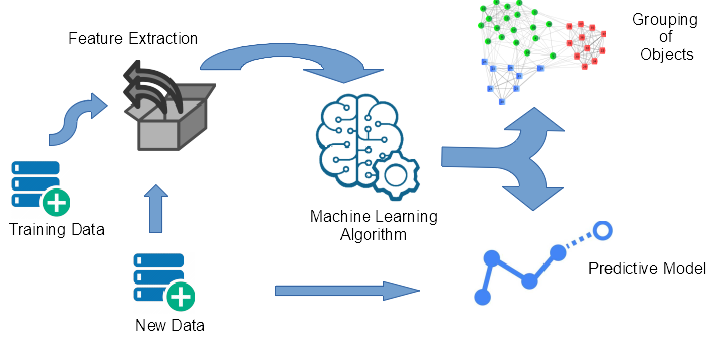
\includegraphics[width=150mm, scale = 1]{images/1_Supervised.png}
	\caption{Supervised Learning Workflow.}
	\label{figure:Supervised_Learning}
\end{figure}

Figure \ref{figure:Supervised_Learning} shows the process of a supervised learning model. The input of the model is data that contains each element with its respective label, next the model extracts the most relevant features of the data, to find the relation between input and output, and construct a logical pattern. Finally, the model after the training step can predict new outputs given a new data without labels.

\subsection{Unsupervised Learning}

Today Big Data is a great tool that makes possible analyze a great amount of information, faster and easier.  Raw data in many cases is difficult to analyze and many cases we do not have an answer key for our trainable data. In this cases we can use unsupervised learning like an alternative, therefore we can determine correlations and identify pattern parsing the available data \cite{Nevala2017}.

This kind of algorithms learns patterns without an explicit feedback (``label'') \cite{Russell2010}, we only have a training data without target values for them \cite{Nilsson1998}. There is no separation of training data and test data \cite{Shai2014}; all the data is the input for the algorithm. Here we have a similitude with the human behavior, when they observe the world, usually they do inferences and group things based on their interaction with the environment, and they are guided by their observations and intuition, this learning is refined exposing to experience and a lot of observations \cite{Nevala2017}.

A the most common technique for this learning is called clustering, \cite{Russell2010} which classify data in meaningful categories, dividing the data into groups with similar characteristics called clusters \cite{Nilsson1998} \cite{Goodfellow2016}. Other techniques are nearest neighbor mapping, singular value decomposition to name a few. Their applications are related to market basket analysis, anomaly/intrusion detection, text classification, identifying like things, sentiment analysis, and so on \cite{Nevala2017} \cite{Halibas2018}.

\begin{figure}[H]	
	\centering
	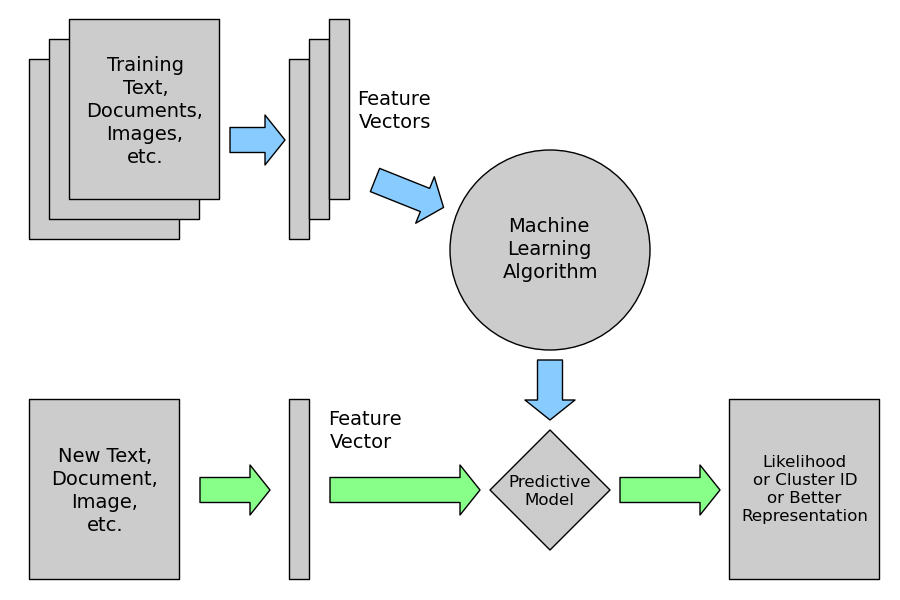
\includegraphics[width=150mm, scale = 1]{images/2-Unsupervised_Learning.png}	
	\caption{Unsupervised Learning Workflow.}	
	\label{figure:Unsupervised_Learning}
\end{figure}

In Figure \ref{figure:Unsupervised_Learning} the features or patterns are extracted of the input data (text, documents, images, etc) data, represented in dimensionality vector, with this data the algorithm is trained. The model created is able use new data to predict outputs like group likelihood or cluster ID.

\section{Neural Networks}
An artificial neural network is a very simplified abstract model of a biological brain, an interconnection of processing units with capability to learn patterns to generalize and associate data. A significant aspect adopted from biological brain is the ``learning capability’’ from the experience and transfer knowledge to find reasonable solutions to similar tasks \cite{ Gurney2004} \cite{ Kriesel2005}.

When we speak about network, it can be referred from a simple single node to a collection of nodes \cite{ Kriesel2005}. The structures of neural networks are basically the next 1) a set of nodes linked associated with a numeric weight that represent the strength of connection between them, 2) an input function for each node that computes the weighted sum of all inputs and 3) an activation function to control the neuron behavior and get the desired output \cite{ Kriesel2005} \cite{Russell2010}. 

\begin{figure}[H]	
	\centering
	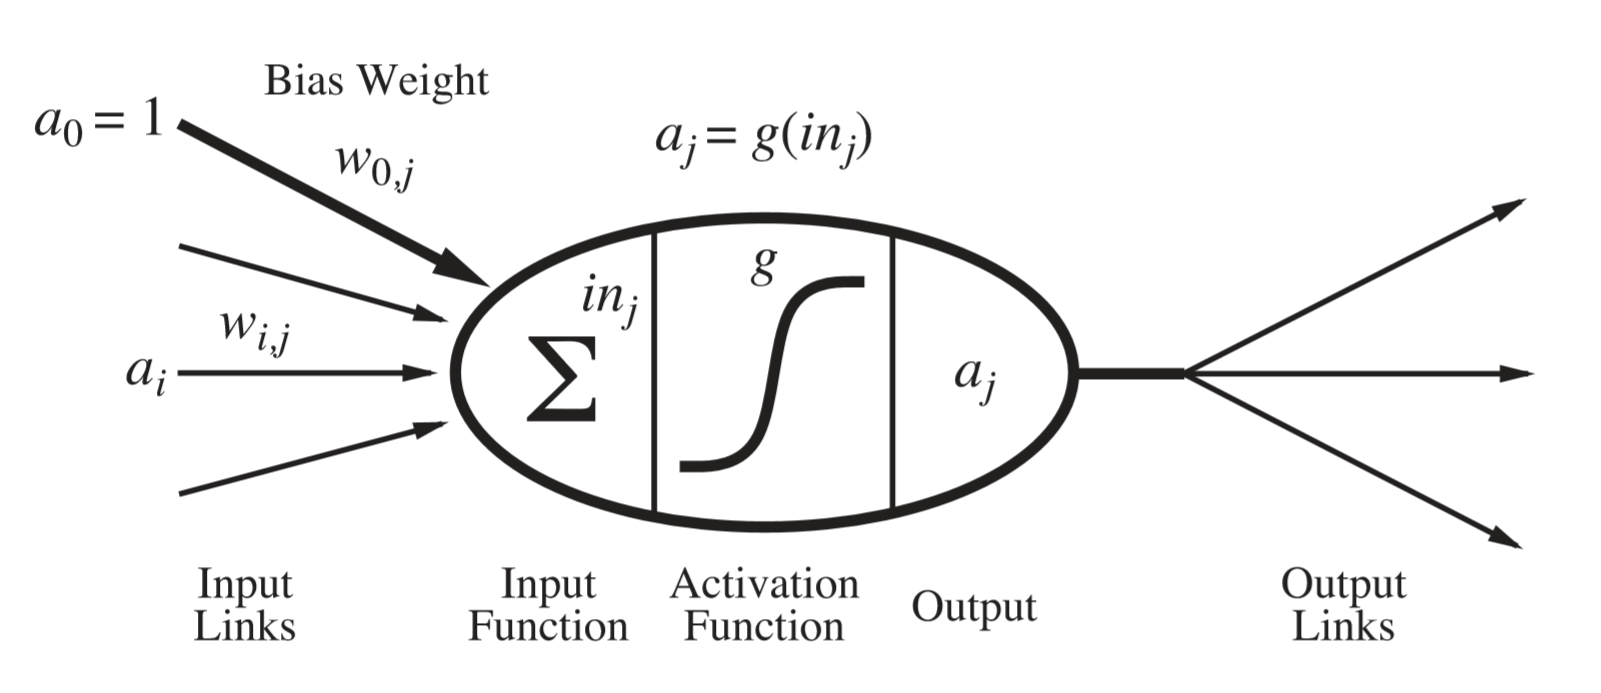
\includegraphics[width=160mm, scale = 1]{images/3_neuron.png}	
	\caption{A Simple Mathematical Neuron Representation \cite{Russell2010}.}	
	\label{figure:Mathematical_Neuron}
\end{figure}

Figure \ref{figure:Mathematical_Neuron} show the basic structure of a simple mathematical neuron, where output is result of apply an activation function (e.g. binary threshold, logistic function, Rectified linear unit function, etc.) to the weighted sum of inputs. The weights are important to minimize the cost of activation function and they are updated when the model is trained. The following equation represent the output after applying an activation function in a neuron showed in Figure \ref{figure:Mathematical_Neuron}.

\begin{equation}
a_j=g\Biggl(\sum_{i=0}^{n} w_{ij}\; a_i\Biggr),
\end{equation}

To form a network, we need connect all these individual neurons like a structure. There are many ways to build the network, feed-forward network and recurrent network are two network topologies very used. The first one showed in Figure \ref{figure:feed-forward-network}, is a network with component clearly separated: an input layer, an output layer and one or more hidden layers also called processing layers. All connections are directed to the following layer and the internal states are just the weights themselves. The second network design the neurons have extra connections adding to a classic feed-forward network, they can be a direct recurrence when the neurons are connected to themselves,  indirect recurrence is a connection to previous layers and a lateral recurrence exist when neurons have connections with another ones at the same layer. These connections influence the neurons itself and their influence depends of the kind of recurrent design. This mean that the network is a dynamic system, the fact that this network feeds its outputs back in its own inputs permit a short-term memory, a model more seem to a brain and by the way, more difficult to understand and build \cite{Kriesel2005} \cite{Russell2010}. 

\def\layersep{5cm}
\begin {figure}[H]
\centering
\resizebox {\textwidth} {!} {
	\begin{tikzpicture}[shorten >=1pt,->,draw=black!100, node distance=\layersep]
	\tikzstyle{every pin edge}=[<-,shorten <=1pt]
	\tikzstyle{neuron}=[circle, fill=red!100, minimum size=20pt,inner sep=0pt]
	\tikzstyle{input neuron}=[neuron, fill=black!100];
	\tikzstyle{output neuron}=[neuron, fill=black!100];
	\tikzstyle{hidden neuron}=[neuron, fill=black!100];
	\tikzstyle{hidden1 neuron}=[neuron, fill=black!100];
	\tikzstyle{annot} = [text width=4em, text centered]
	
	% Draw the input layer nodes
	\foreach \name / \y in {1,...,3}
	\node[input neuron] (I-\name) at (0,-2*+\y) {};
	
	% Draw the hidden layer nodes
	\foreach \name / \y in {1,...,8}
	\path[yshift=0.5cm]
	node[hidden neuron] (Hb-\name) at (\layersep,-\y cm) {};
	
	\foreach \name / \y in {1,...,8}
	\path[yshift=0.5cm]
	node[hidden neuron] (H-\name) at (2*\layersep,-\y cm) {};
	
	\foreach \name / \y in {1,...,8}
	\path[yshift=0.5cm]
	node[hidden neuron] (Ha-\name) at (3*\layersep,-\y cm) {};
	
	
	% Draw the output layer node
	%\node[output neuron,pin={[pin edge={->}]right:Output}, right of=H-3] %(O) {};
	\foreach \name / \y in {1,...,2}
	\path[yshift=0.5cm]
	node[hidden neuron] (o-\name) at (4*\layersep,-3*\y cm) {};
	
	% Connect every node in the input layer with every node in the
	% hidden layer.
	\foreach \source in {1,...,3}
	\foreach \dest in {1,...,8}
	\path (I-\source) edge (Hb-\dest);
	
	\foreach \source in {1,...,8}
	\foreach \dest in {1,...,8}
	\path (Hb-\source) edge (H-\dest);
	
	\foreach \source in {1,...,8}
	\foreach \dest in {1,...,8}
	\path (H-\source) edge (Ha-\dest);
	
	% Connect every node in the hidden layer with the output layer
	\foreach \source in {1,...,8}
	\foreach \dest in {1,...,2}
	\path (Ha-\source) edge (o-\dest);
	
	% Annotate the layers
	\node[annot,above of=H-1, node distance=1.5cm] (hl) {Hidden layers};
	\node[annot,above of=I-1, node distance=3.2cm] (il) {Input layer};
	\node[annot,above of=o-1, node distance=3.2cm] {Output layer};
	\end{tikzpicture}
}
\caption{Feed Forward Network}
\label{figure:feed-forward-network}
\end{figure}


\section{Deep Learning with Neural Networks}

The artificial intelligence usually solves problems intellectually challenge for the humans relatively easy, but the task the human performs easy or solve intuitively are very difficult for the computers. The problems like speech recognition or applications to find faces in images are challenge task. For these problems we must allow computers gather knowledge from the experience, avoiding specify all the knowledge that the system needs. It means build a complicated task using simpler concepts \cite{Goodfellow2016}.

This approach is a \ac{ML} modern and advanced technique, the base in many advances of  \ac{AI} fields, like Natural Language Processing, Speech Recognition, Computer Vision, Biomedical Applications and so on; using the most sophisticated neural networks. These models form a complex and deeper graph than a normal neural network, including many layers and neurons, this is why we know this approach as Deep Learning \cite{Chandra2017} \cite{Goodfellow2016} \cite{Nevala2017}.

The most typical example of \ac{DL} approach is feed-forward deep network. It consists in an input layer, that contains the input data for the model, next we have the hidden layers, a variable number of neurons and layers, and finally an output layer as is showed in the Figure \ref{figure:feed-forward-network}. That depth (number of hidden layers) allows to learn a multi-step program. There are many algorithms of \ac{DL}, like \ac{CNN} used commonly when is working with images and \ac{RNN} to process sequences of data. 

\subsection{Fully Connected Networks}
These networks are a traditional full connected feed-forward network with many layers fully connected, it means all nodes from a layer relate to all nodes of following layer and same way for the other layers. This network is a little similar to \ac{CNN} but could be computationally expensive. With modern hardware and specially using \ac{GPU} is possible achieve tasks successfully. Today we know that is not necessary to train a fully connected deep architectures due the resources that needs, but they were the first to be succeed \cite{Goodfellow2016}.

\subsection{Convolutional Neural Networks}
This kind of networks is applied to problems with a grid-like topology, a clear example of this type of data are the images, other are the regular time intervals. \ac{CNN} formally is composed with a mathematical operation called convolution in at least one layer, instead of a general matrix operation \cite{Goodfellow2016}. This kind of algorithm is very used in pattern recognition, as a powerful visual model, to extract features in a hierarchy of concepts. \cite{Long2015}. Historically this type of network was some the firsts in solve important commercial problems \cite{Goodfellow2016}, like the handwritten zip code recognition.

\subsection{Recurrent Neural Networks}
In other hand \ac{RNN}, is a kind of networks to processing sequential data. They are very powerful because they store efficiently information about the past. They are specialized in process a sequence of values \cite{Goodfellow2016}, mapping all the previous input to each output. This allows the memory of old inputs can persist and influence in the next network output \cite{Graves2017}. \ac{RNN} are used for resolving many types of problems, \cite{Chandra2017} proposes a method to improving the use of this algorithm in classification of images. Other applications are sentimental classification, topic classification, summarization and machine translation.

Train a \ac{RNN} for task that need information over the time is not easy, because a simple network do not maintain contextual information distant from the current step of processing. To do these kinds of task is necessary implement network more complex for maintain information as needed for future steps and remove which are not necessary \cite{Jurafsky2018}. The network more known with this type of design are \ac{LSTM} and \ac{GRU} that are described following.


\subsubsection{Long Short-Term Memory}
This network manages the contextual information forgetting the information that is not useful and maintaining the information that have more probability to be used in next processes. The training task is specialized in achieve a better manage of contextual information to discard it or save it. To control the flow of information over the gates of the network exist a specialized neural unit to control the input and output of the information \cite{Jurafsky2018}.

\subsubsection{Gated Recurrent Unit}
This kind of network is an easier way to implement a recurrent network with control of memory, it means than is a special case of a \ac{LSTM}, where instead to introduce a lot of input parameters here, this network use a single ``gate'' to set weights and update parameters. These neural units are more complex that the basic feed-forward network units, but they are largely encapsulated with the basic units, maintaining the modularity and making easier to experiment with these kind of architectures \cite{Jurafsky2018}.

\section{Natural Language Processing}

\ac{NLP} is the process to understand, analyze and use of human language by machines or algorithms, this comprehends the written text, voice commands or both, to draw insight, advertisement, and so on. There is many information in web pages and almost all of them are in natural language, one reason why we want our algorithms can understand human language is to acquire information from written and spoken language. An algorithm that wants acquire knowledge needs to comprehend at least partially the human language use (e.g. ambiguity and messy). This undertaking is not trivial because the presence of the colloquialism, figure of speech, abbreviations, emoticons to mention a few \cite{Nevala2017} \cite{Russell2010}. The difference with a formal language (e.g. python or java) is that a natural language cannot be characterize in a set of sentences, because they are very large, ambiguous and constantly changing; the our best model is just an approximation \cite{Russell2010}.

The process of language analysis is closely related to linguistic, traditionally, this process is decomposed in three stages: syntax, semantic and pragmatics; we first analyze the syntaxis of a text providing an order and a structure and then to analyze in terms of meaning (semantic), and last stage is an pragmatic analysis, who relates the sentence with a context. Such separations constitute the basis for architectural models from a software point of view, making the analysis more manageable and serving like a starting point. Recently the decomposition of this process and needs to work with real language data has change the schema \cite{Indurkhya2010}, like is showed in Figure \ref{figure:NLP_Stages}.

\begin{figure}[H]	
	\centering
	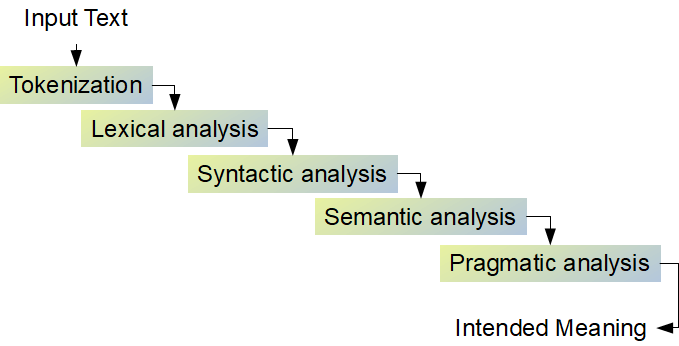
\includegraphics[width=150mm, scale = 1]{images/4_nlp.png}	
	\caption{Natural Language Process Stages}	
	\label{figure:NLP_Stages}
\end{figure}

Figure \ref{figure:NLP_Stages} represent the stages in a \ac{NLP}, 1) tokenization is about divide a continuous text data in words or sentences, in English is usually separated by whitespaces but other unsegmented languages is more complicated to do, because there is not a visible separation between words (e.g. Chinese, Japanese) that need more than a simple lexical analysis. 2) lexical analysis refers to morphological processing, mapping strings to lemma and assigning structure to words and registering their structural properties. 3) syntactic analysis is analyzing a sentence and determine its structural composition following rules of a formal grammar (grammar formalism to describe language syntax) to finally assign a meaning to the sentence. The syntax tree is the standard to represent a syntactic structure which contains the steps in the derivation from the main node. 4)semantic analysis is related with the context of languages (words, phrases, scenarios, etc.), this not only refers to meaning of a sentence, but also to its relationship with others words or sentences, that means to simulate the inferencing process and achieve a better interaction between a human and a machine.  5)pragmatic analysis also called natural language generation is the process when a machine has to say something, the thought has to render in a language with the intention to communicate something with a correct context (it depends of the program goals) \cite{ Indurkhya2010}.

Applications of \ac{NLP} are based on probability distributions over sequential data in a natural language, we can use generic neural networks for basic tasks, however in complex applications we need specialized techniques to process data, sometimes we regard like a sequence of words, characters or even bytes. The earliest successful language model, a probability distribution over sequential data, was n-gram models (sequences of tokens). It has many possible types: unigrams, bigram, trigram, n-gram; to improve statistical efficiency was introduced the notion of word categories or class-based n-grams models, however they are not able to share statistical strength of similar words and their contexts. Here appears the neural languages model that could recognize the similarity not only between words but also in their contexts for each one. This distributed representation sometimes is called word representation or word embedding, that means the language symbols are represented as points in a space dimension. In an embedding space, words with similar meaning are close each other \cite{Russell2010} \cite{Goodfellow2016}. The most known word representation are Word2Vec Model, an improve of skip-gram model in terms of quality of vectors and speed training \cite{Mikolov2013} and GloVe model that combines the advantages of global matrix factorization and local context window \cite{Pennington2014}. More recent studies show other sentences encoder like Skip-Thought Vectors, an approach for unsupervised learning that tries to reconstruct passages of text that share semantic properties \cite{Kiros2015}, Supervised Learning of Universal Sentence Representations from Natural Language Inference Data, an encoder using pre-trained sentence level embedding with supervised data of Stanford Natural Language Inference datasets demonstrating stronger transfer task than skip-thought vectors \cite{ Conneau2017}. Universal Sentence Encoder, other encoder that use supervised data to train a sentence embedding model instead a word level embedding, showing a good performance \cite{Cer2018}. 

There are several applications of \ac{DL} techniques in \ac{NLP} task including:

\begin{itemize}[nolistsep]
	\item \textbf{Spelling and Grammar Checking:} The suggestions that appear when we type a text in a smartphone or when we redact a document in an advance text editor. 
	
	\item \textbf{Text Classification:} It is the categorization of a text in a defined set of classes, language identification and spam detection are examples of text classification \cite{Russell2010}.
	
	\item \textbf{Information Retrieval:} When the algorithm results a set of documents responding to a query like the search engines does \cite{Russell2010}.
	
	\item \textbf{Summarization:} To obtain the essential information from a long document in a shorter piece of text.
	
	\item \textbf{Syntactic Analysis:} It consists in analyze a string of words to isolate subjects, verbs, adverbs, adjectives and others complements (phrase structure) \cite{Russell2010}.
	
	\item \textbf{Machine Translation:} It is the task to automatic translation an equivalent sentence in meaning in another natural language \cite{Goodfellow2016}.
	
	\item \textbf{Speech Recognition:} This task identifies the words given by a speaker. That is difficult because the ambiguity and noisy are a hard challenge \cite{Russell2010}.
	
\end{itemize}

\section{Text Similarity}
Text similarity refers to how close is a text whit another one in terms of meaning and surface closeness, the first means semantic similarity and the last is called lexical similarity. All works in lexical similarity often are developed to achieve to semantic similarity \cite{Ganesan2015}. Similarity refers to the measure of the relationship between two pieces of text, this similarity is defined lexically or semantically. Lexical similarity exists when there is character or word matching (e.g. ``feel'' and ``feet''), in other hand semantic similarity is based on meaning and context (e.g. ``Long Short-Term Memory'' and ``\ac{LSTM}'') \cite{Pradhan2015}. 
Text similarity is involve in many text research such as text classification, clustering, information retrieval, topic detection, machine translation, summarization and others \cite{Majumder2016} \cite{Gomaa2013} \cite{Pradhan2015}, where most of these are related with social network analysis \cite{Zhang2015}.  

\subsection{Lexical Similarity}
When we talk about of lexical similarity, it refers to found same words or characters in the evaluation sentences (matching or comparison). Hence in this kind of similarity, the meaning is not known then we can use lexical analysis techniques to achieve better accuracy, for example we can add no-determiner words to expand the scope and provide some of context \cite{Ganesan2015} \cite{Gomaa2013}. This metric could be used on clustering, redundancy removal and information retrieval \cite{Ganesan2015}. Lexical similarity could categorize depending of the granularity used. It can be character level, word level or phrase level \cite{Ganesan2015} \cite{Pradhan2015}. String-based methods to calculate the measure of similarity are categorized as follows

\begin{itemize}[nolistsep]
	\item \textbf{Character based similarity:} There are many techniques of measure based on characters, longest common substring/subsequence is a method that find substring and compare based in common chain of characters that both share, this is the longest common chain of suffixes for each substring. Levenshtein distance, where the measure is given by the number of operations to transform one string in another one, using insertions, deletion or substitution of adjacent characters. Other method is Jaro distance that emphasize in the number and order of matching common characters, it is used in duplicate detection (record linkage). Finally, n-gram method that calculate the distance of two sub sequences, dividing its similar n-grams by maximal number of n-grams. These methods are not the unique, exist others like Jaro-Winkler, Needleman-Wunsch, Smith-Waterman and Syntactic n-gram to mention a few \cite{Gomaa2013} \cite{Majumder2016} \cite{Pradhan2015}.
	\item \textbf{Statement/Term based similarity:} A method widely knows in text similarity is cosine similarity, where the distance is given by the cosine of the angle between two vectors in an inner product space, these vectors represent the sentences. Euclidean distance also called L2 distance use vectors in a Euclidean space where the distance is the square root of the sum of squared difference between two vectors (sentences). Jaccard similarity coefficient or Jaccard index is used to calculate similarity and diversity in sets, it takes the shared term in the intersection and it is divided by number of all terms of the union. There are other known methods like block distance (Manhattan distance, L1 distance, etc.), Dice's Coefficient, Matching coefficient, overlap coefficient, soft-cosine similarity, centroid based similarity and others\cite{Majumder2016} \cite{Pradhan2015} \cite{Gomaa2013} .
\end{itemize}

\subsection{Semantic Similarity} \label{sem_sim}
One field mostly studied in similarity, is about measures of similarity that they have in mind the meaning and context of sentences that even could be syntactically very similar. Semantic analysis entails a deeper level of analysis, for example syntactic parsing to get dependency structure in the phrases. Commonly semantic similarity use background information about concepts like WordNet, Wikipedia and so on or an simplify corpora of a texts collection \cite{Ganesan2015} \cite{ Zhang2015}.
Semantic similarity is frequently used for text summarization, topic analysis, recommendation system, collaborative tagging system and others. This approach could be classified in three big categories based in the use of information: corpus based,  knowledge based and hybrid methods \cite{Gomaa2013} \cite{Zhang2015}. These categories are described below.

\begin{itemize}[nolistsep]
	\item \textbf{Corpus based similarity:} 
	Also called statistical similarity, this approach refers in use information gathered from a large corpus from written o spoken data. Latent semantic analysis represents the text in a matrix where rows are the unique words and columns represent each sentence. This method is constructed based in a corpus of text and a mathematical technique called singular value decomposition to reduce dimensionality maintaining similarity relation between word and text. To calculate the similarity often is used cosine similarity.  Other technique is hyperspace analogue to language, it is a variation of latent semantic analysis, taken a set of words called a ``window'' and is compare with the corpus to calculate co-occurrences in words, forming a matrix representing the strength between related words. Its similarity also can measure with cosine similarity method. Explicit semantic analysis uses the Wikipedia corpus to convert sentences in a tf-idf (term-frequency-inverse document frequency) weighted vector between each word and the documents of corpus. The measure to calculate the distance between vector is cosine similarity. Normalize Google distance is a semantic metric that use Google search to get the number of hits returned for each term of the text and build a metric to calculate the words with similar meaning between two sentences. Other methods are point wise mutual information, normalize information distance, normalize compression distance and so on \cite{Ganesan2015} \cite{ Zhang2015} \cite{Gomaa2013} \cite{Majumder2016}.
	
	\item \textbf{Knowledge based similarity:} It is called topological similarity and it is based in semantic networks, these networks are a lexical database grouped in set of semantic synonyms with conceptual and lexical relation that include verbs, nouns, adverbs and adjectives. The most popular semantic networks are Word Net and Natural Language Toolkit \cite{gomaa2013} \cite{Pradhan2015} \cite{Majumder2016}. There are distinct types of categorization for this kind of similarity measure focused in similarity or relatedness. Some authors divide it in the following types: \textit{Node-based} (also called information content based) similarity that calculate the similarity between two sentences by the amount of information that share each other, one method very used in this approach is Resnik similarity method, it uses only Word Net nouns to get the information content of sentences, other measures are Lin method, Jiang and Conrath method \cite{Majumder2016} \cite{Zhang2015} \cite{Pradhan2015}. \textit{Edge based} approach counts the edges of graphs (semantic network) between the compared concept nodes where nodes with shorter path are more similar. All edges are weighted considering network density, node depth, type of link and link strength \cite{Majumder2016}  \cite{Zhang2015}. Other approach is \textit{feature based}, it uses the concepts of Word Net as a list of features to calculate the semantic similarity between sentences \cite{Zhang2015}, and finally \textit{gloss based} approach uses glosses of words from a given corpus. One method in this group is, Vector Measure, it forms a co-occurrence matrix with the average of each co-occurrences vector of a gloss/concept to measure the semantic similarity \cite{Pradhan2015}  \cite{Zhang2015}.
	
	\item \textbf{Hybrid similarity measures:} This approach refers to use the best of above two categories and others, like lexical structure and corpus information, combining several metrics into one. For example, semantic text similarity method is combination of syntactic and semantic information \cite{Zhang2015} \cite{Gomaa2013}. Other methods combine more approaches, \cite{Zhu2014} built a supervised random forest regression model that use machine learning methods to combine string features, corpus-based methods, knowledge-based method, syntactic features, multi-level text features and so on.
	
\end{itemize}

\chapter{Problem Formulation} \label{chapter 3}
\section{Description}
The main problem tackled in this project is to achieve to use the \ac{THS} data to train an algorithm able to identify the similarity between two sentences (tweets). This will allow us setup a process to watch the Twitter stream and collect similar tweets to these one and present these tweets to the user sorted by relevance of their similarity. As we describe in section \ref{sem_sim}, the similarity is very difficult to calculate due to is hard to find the meaning and context macth of the two pieces of text. To manage those issues, we use relevant information to find context similarity and syntactical similarity, like the type of disease mentioned on each sentence or if they are related to a disease or not, and a metric that describe the level of similarity between tweet texts, that are tagged in a range of one to four, where one is less similar and four is more semantically similar.

Following we describe some samples of tweet sentences with a previous pre-processing to show the complexity of work with data related to semantic measures and contextual similarity.

\begin{definition} Tweets no related – Different diseases.
	\begin{itemize}[nolistsep]
		\item Measles starts with cold like symptoms that develop about of days after becoming infected this is followed a few days later by the measles rash poster shows us the symptoms to look out for think measles prevention is best a dose of vaccine needed vaccines work.
		\item The Ebola outbreak was a worst nightmare for countries affected interestingly Ebola was not a new disease in fact on managing the disease there is a forty year old knowledge so how did Ebola become such an epidemic.
	\end{itemize}
\end{definition}
In this example, the two tweets speak about diseases, one of them describe the symptoms of measles and recommend the prevention using vaccines. The other one does a question about the reason why Ebola were expanded if this disease is not new and there is enough knowledge about it.  The content of these two sentences are related with a health condition but they are describing different diseases, that is enough to consider it no similar.

\begin{definition} Tweets no related – Same disease.
	\begin{itemize}[nolistsep]
		\item Theory man flu exists as a phenomenon because it is the only time toxic masculinity tells men it is okay to feel vulnerable weak and look to their partners for support.
		\item yeah, I missed like a day of school on and off flu I could not even eat, and I could not walk without feeling like vomiting or collapsing.
	\end{itemize}
\end{definition}
The first tweet refers to flu, but it is not about a condition health, in change is an assumption about the flu exists to show the vulnerability weak of men over their partners. I other hand the second one speaks about someone that missed a school day because flu and speak about his/her symptoms.


\begin{definition} Tweets related – Same diseases.
	\begin{itemize}[nolistsep]
		\item I wish I knew if the twins were going to get the flu like what is the usual window, he is had it symptom wise since Sunday night and it is Tuesday so when would they likely show symptoms ahh.
		\item So I was at the hospital and obviously could not type while I was there since, a I could not type and b I was scared of being caught with lewd rps after I healed bad luck struck again and I was bedridden with the flu all I did was sleep and I was coughing so much my eyes went red.
	\end{itemize}
\end{definition}
In this case the first tweet tells about twins getting flu and describe the intervals of days with possible symptoms. The second is about a person that who was in the hospital and explain that was the reason because she/he could not type, and when he or she was recuperated then got flu again and just goes to sleep. The two sentences are showing a health condition (flu) where the writers are explaining symptoms and what they were doing when they got flu. Therefore, these sentences are related.

\section{Formalization}
\section{Data Processing Architecture}

\begin{figure}[H]	
	\centering
	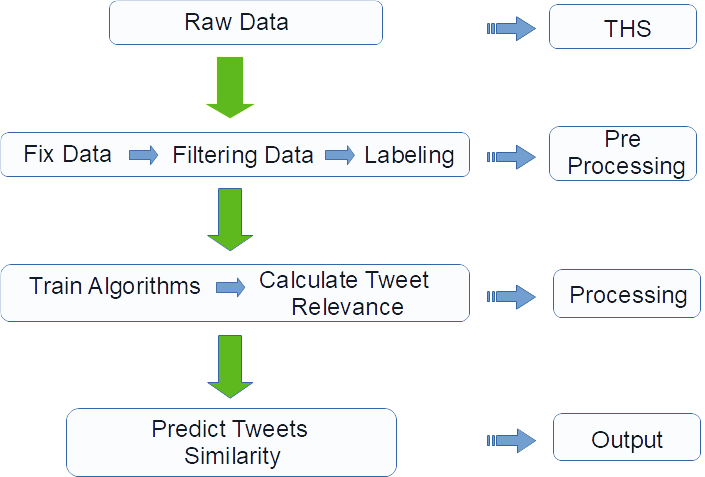
\includegraphics[width=150mm, scale = 1]{images/5_data_processing.png}	
	\caption{Data Processing Architecture}	
	\label{figure:data_processing}
\end{figure}

The architecture of tweet processing is showed in Figure \ref{figure:data_processing}. Tweets were collected in \ac{THS} system in a distributed system database over \ac{HDFS}. Tweets selected was cleaned, removing links, hashtags and mentions. In a next stage the text passes through a pre-processing expanding contractions and correcting misspelling.

Next stage tweets are filtered to associate to a disease. After detecting if the text is related to a disease, tweets are labeled to know if each tweet is speaking about a disease or if it is a lexical or semantical ambiguity. Other process to prepare the data to training is take an average measure of three labelers about the level of similarity between tweets as part of pre-processing stage.

The previous stages are the input of the main process to train algorithms and calculate tweets relevance and after to present these tweets to the user sorted by relevance of their similarity as the output of the model.

\chapter{System Architecture and Organization} \label{chapter 4}
\section{THS System Overview}
Text here
\section{How to Define Similarity}
\section{Model Learning Architecture}
\subsection{Neural Networks used for Learning Similarity}
\subsection{Neural Networks Variations}

\chapter{Performance Evaluation} \label{chapter 5}
\section{Hardware} 
\section{Software}
\section{Experiment Setup}
\section{Data Collection}
\section{Data Labeling}
\section{Data Pre-processing}
\section{Experimental Results and Discussion}

\chapter{Conclusion and Future Work} \label{chapter 6}
In summary, text here

%\chapter*{References} 
%\addcontentsline{toc}{chapter}{Bibliography}
\bibliographystyle{unsrt}
\bibliography{references} 
%\printbibliography[heading=none, ]

\begin{appendices}
\chapter{GitHub Repositories}
The GitHub repositories of the big data and machine learning deamon are avaliable upon request at danny.villanueva1@upr.edu. The following sections contain the links.

\section{Big Data Platform}
https://github.com/THSUPRM/bigdata/tree/master/python

\subsection{Machine Learning Platform}
https://github.com/THSUPRM/bigdata/tree/master/DetectDiseaseTHS/ths
\end{appendices}

\end{document}